\documentclass{article}
\usepackage{v-test-paper}
\newenvironment{solution}{\par\noindent\color{red!85!black}$\Rightarrow$\vspace{0em}}{}
\title{\textsc{JEE Advanced 2012 Paper-I\\Physics}}
\date{}
\begin{document}
\maketitle
\begin{enumerate}
    
\item At time \( t = 0 \), terminal A in the circuit shown in the figure is connected to B by a key and an alternating current \( I(t) = I_0\cos(\omega t) \), with \( I_0 = 1 A \) and \( \omega = 500 \text{ rad s}^{-1} \) starts flowing in it with the initial direction shown in the figure. At \( t = \frac{7\pi}{6\omega} \), the key is switched from B to D. Now onwards only A and D are connected. A total charge \( Q \) flows from the battery to charge the capacitor fully. If \( C=20\mu F \), \( R=10 \Omega \) and the battery is ideal with \( emf \) of \( 50 V \), identify the correct statement(s).
    \begin{center}
        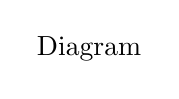
\begin{tikzpicture}
            \node at (0, 0) {Diagram};
        \end{tikzpicture}
    \end{center}
    \begin{tasks}(2)
        \task Magnitude of the maximum charge on the capacitor before \( t = \frac{7\pi}{6\omega} \) is \( 1 \times 10^{-3} C \).
        \task The current in the left part of the circuit just before \( t = \frac{7\pi}{6\omega} \) is clockwise.
        \task Immediately after A is connected to D, the current in \( R \) is \( 10 A \).
        \task \( Q = 2 \times 10^{-3} C \).
    \end{tasks}

    
\item A real gas behaves like an ideal gas if its
    \begin{tasks}(2)
        \task pressure and temperature are both high
        \task pressure and temperature are both low
        \task pressure is high and temperature is low
        \task pressure is low and temperature is high\ans
    \end{tasks}

    
\item A car starts moving rectilinearly, first with acceleration $w = -5.0\ m/s^2$ (the initial velocity is equal to zero), then uniformly, and finally, decelerating at the same rate $w$, comes to a stop. The total time of motion equals $\tau = 25\ s$. The average velocity during that time is equal to $\langle v \rangle = 72\ km$ per hour. How long does the car move uniformly?

    \item Given below are two statements:\\
\textbf{Statement I}: An elevator can go up or down with uniform speed when its weight is balanced with the tension of its cable.

\textbf{Statement II}: Force exerted by the floor of an elevator on the foot of a person standing on it is more than his/her weight when the elevator goes down with increasing speed.

In the light of the above statements, choose the correct answer from the options given below:
\begin{tasks}(1)
    \task Statement I is false but Statement II is true
    \task Both Statement I and Statement II are true
    \task Both Statement I and Statement II are false
    \task Statement I is true but Statement II is false
\end{tasks}
    
\item A point source $S$ is placed at the bottom of a transparent block of height $10\ mm$ and refractive index $2.72$. It is immersed in a lower refractive index liquid as shown in the figure. It is found that the light emerging from the block to the liquid forms a circular bright spot of diameter $11.54\ mm$ on the top of the block. The refractive index of the liquid is
    \begin{center}
        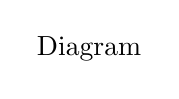
\begin{tikzpicture}
            \node at (0, 0) {Diagram};
            % Note: The actual diagram should replace this placeholder
        \end{tikzpicture}
    \end{center}
    \begin{tasks}(2)
        \task \(1.21\)
        \task \(1.30\)
        \task \(1.36\)
        \task \(1.42\)
    \end{tasks}

    
\item Consider a disc rotating in the horizontal plane with a constant angular speed $\omega$ about its centre $O$. The disc has a shaded region on one side of the diameter and an unshaded region on the other side as shown in the figure. When the disc is in the orientation as shown, two pebbles $P$ and $Q$ are simultaneously projected at an angle towards $R$. The velocity of projection is in the $y$-$z$ plane and is same for both pebbles with respect to the disc. Assume that (i) they land back on the disc before the disc has completed $\frac{1}{8}$ rotation, (ii) their range is less than half the disc radius, and (iii) $\omega$ remains constant throughout. Then
    \begin{center}
        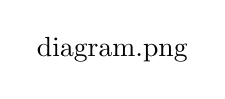
\begin{tikzpicture}
            \node at (0, 0) {diagram.png};
        \end{tikzpicture}
    \end{center}
    \begin{tasks}(1)
        \task $P$ lands in the shaded region and $Q$ in the unshaded region.
        \task $P$ lands in the unshaded region and $Q$ in the shaded region.
        \task Both $P$ and $Q$ land in the unshaded region.
        \task Both $P$ and $Q$ land in the shaded region.
    \end{tasks}

    \item Ratio of thermal energy released in two resistors \(R\) and \(3R\) connected in parallel in an electric circuit is :
\begin{tasks}(2)
    \task \(1 : 1\)
    \task \(1 : 27\)
    \task \(1 : 3\)
    \task \(3 : 1\)
\end{tasks}
    
\item A spherical metal shell A of radius $R_A$ and a solid metal sphere B of radius $R_B$ ($R_B < R_A$) are kept far apart and each is given charge $`+Q'$. Now they are connected by a thin metal wire. Then
    \begin{tasks}(2)
        \task $E_{\text{inside}}^A = 0$
        \task $Q_A > Q_B$
        \task $\frac{\sigma_A}{\sigma_B} = \frac{R_B}{R_A}$
        \task $E_{\text{on surface}}^A < E_{\text{on surface}}^B$
    \end{tasks}

    \item A bar of mass \( m \) is pulled by means of a thread up an inclined plane forming an angle \( \alpha \) with the horizontal (Fig. 1.13). The coefficient of friction is equal to \( k \). Find the angle \( \beta \) which the thread must form with the inclined plane for the tension of the thread to be minimum. What is it equal to?
    \begin{center}
        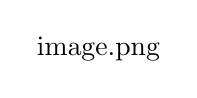
\begin{tikzpicture}
            \node at (0, 0) {{image.png}};
        \end{tikzpicture}
    \end{center}
\begin{solution}
    \begin{center}
        \begin{tikzpicture}
            \pic at (0, 0) {frame=3cm};
        \end{tikzpicture}
    \end{center}
    
    \begin{align*}
        \intertext{Let us fix the $x - y$ co-ordinate system to the wedge, taking the $x$-axis up along the incline and the $y$-axis perpendicular to it (see figure).}
        \intertext{Now, we draw the free body diagram for the bar.}
        \intertext{Let us apply Newton’s second law in projection form along $x-$ and $y-$axes for the bar}
        T \cos \beta - mg \sin \alpha - fr &= 0 \tag{1}\\
        T \sin \beta + N - mg \cos \alpha &= 0 \tag{2}
        \intertext{or $N = mg \cos \alpha - T \sin \beta$}
        \intertext{But, $fr = kN$ and using Eq. (2) in Eq. (1), we get}
        T &= mg \sin \alpha + kmg \cos \alpha / (\cos \beta + k \sin \beta) \tag{3}
        \intertext{For $T_{\min}$ the value of $(\cos \beta + k \sin \beta)$ should be maximum}
        \frac{d (\cos \beta + k \sin \beta)}{d\beta} &= 0 \quad \text{or}\quad \tan \beta = k
        \intertext{Putting this value of $\beta$ in Eq. (3), we get}
        T_{\min} &= \dfrac{mg \left( \sin \alpha + k \cos \alpha \right)}{\sqrt{1+k^{2}}}
    \end{align*}
\end{solution}

    
\item Two bodies were thrown simultaneously from the same point: one, straight up, and the other, at an angle of $\theta = 60^\circ$ to the horizontal. The initial velocity of each body is equal to $v_0 = 25$ m/s. Neglecting the air drag, find the distance between the bodies $t = 1.70$ s later.

    
\item A point mass of \(1 \, \text{kg}\) collides elastically with a stationary point mass of \(5 \, \text{kg}\). After their collision, the \(1 \, \text{kg}\) mass reverses its direction and moves with a speed of \(2 \, \text{ms}^{-1}\). Which of the following statement(s) is (are) correct for the system of these two masses?
    \begin{tasks}(2)
        \task Total momentum of the system is \(3 \, \text{kg ms}^{-1}\)
        \task Momentum of \(5 \, \text{kg}\) mass after collision is \(4 \, \text{kg ms}^{-1}\)
        \task Kinetic energy of the centre of mass is \(0.75 \, \text{J}\)
        \task Total kinetic energy of the system is \(4 \, \text{J}\)
    \end{tasks}

    
\item In plotting stress versus strain curves for two materials \(P\) and \(Q\), a student by mistake puts strain on the \(y\)-axis and stress on the \(x\)-axis as shown in the figure. Then the correct statement(s) is(are)
        \begin{tasks}(2)
            \task \(P\) has more tensile strength than \(Q\)
            \task \(P\) is more ductile than \(Q\)
            \task \(P\) is more brittle than \(Q\)
            \task The Young's modulus of \(P\) is more than that of \(Q\)
        \end{tasks}
    \begin{center}
        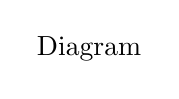
\begin{tikzpicture}
            \node {Diagram};
        \end{tikzpicture}
    \end{center}

    
\item A particle of mass \( M \) and positive charge \( Q \), moving with a constant velocity \( \vec{u}_1 = 4\hat{i} \, \text{ms}^{-1} \), enters a region of uniform static magnetic field normal to the \( xy \)-plane. The region of the magnetic field extends from \( x = 0 \) to \( x = L \) for all values of \( y \). After passing through this region, the particle emerges on the other side after 10 milliseconds with a velocity \( \vec{u}_2 = 2(\sqrt{3}\hat{i} + \hat{j}) \, \text{ms}^{-1} \). The correct statement(s) is (are)
    \begin{tasks}(2)
        \task The direction of the magnetic field is \(-z\) direction.
        \task The direction of the magnetic field is \(+z\) direction.
        \task The magnitude of the magnetic field is \( \frac{50 \pi M}{3Q} \) units.
        \task The magnitude of the magnetic field is \( \frac{100 \pi M}{3Q} \) units.
    \end{tasks}

    
\begin{enumerate}
    \item In the balanced condition, the values of the resistances of the four arms of a Wheatstone bridge are shown in the figure below. The resistance \( R_3 \) has temperature coefficient \( 0.0004 ^\circ C^{-1} \). If the temperature of \( R_3 \) is increased by \( 100^\circ C \), the voltage developed between \( S \) and \( T \) will be \_\_\_\_\_\_\_ volt.
    \begin{center}
        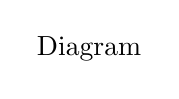
\begin{tikzpicture}
            \node {Diagram};
        \end{tikzpicture}
    \end{center}
\end{enumerate}

    
\item In the given circuit, the AC source has $\omega = 100\ \text{rad/s}$. Considering the inductor and capacitor to be ideal, the correct choice(s) is(are)
    \begin{center}
        \begin{circuitikz}[american]
            \draw (0,0)
            to[V, V=$20\ V$] (0,2) % The voltage source
            to[L, L=$0.5\ H$] (2,2) % The inductor
            to[C, C=$100\ \mu F$] (4,2) % The capacitor
            to[R, R=$100\ \Omega$] (4,0) % 100 ohm resistor
            -- (0,0);
            \draw (2,2)
            to[R, R=$50\ \Omega$] (2,0); % 50 ohm resistor
        \end{circuitikz}
    \end{center}
    \begin{tasks}(1)
        \task The current through the circuit, $I$ is $0.3\ A$.
        \task The current through the circuit, $I$ is $0.3\sqrt{2}\ A$.
        \task The voltage across $100\ \Omega$ resistor is $10\sqrt{2}\ V$.
        \task The voltage across $50\ \Omega$ resistor is $10\ V$.
    \end{tasks}

    \item A planet of mass \( M \), has two natural satellites with masses \( m_1 \) and \( m_2 \). The radii of their circular orbits are \( R_1 \) and \( R_2 \) respectively. Ignore the gravitational force between the satellites. Define \( v_1 \), \( L_1 \), \( K_1 \) and \( T_1 \) to be, respectively, the orbital speed, angular momentum, kinetic energy and time period of revolution of satellite 1; and \( v_2 \), \( L_2 \), \( K_2 \) and \( T_2 \) to be the corresponding quantities of satellite 2. Given \( m_1/m_2 = 2 \) and \( R_1/R_2 = 1/4 \), match the ratios in List-I to the numbers in List-II.

\begin{center}
    \renewcommand{\arraystretch}{2.5}
    \begin{table}
        \centering
        \begin{tabular}{p{0.25cm}p{6cm}|p{0.25cm}p{6cm}}
        \hline
        & List-I & &List-II \\
        \hline
        P. & \( \frac{v_1}{v_2} \) & 1. & \( \frac{1}{8} \) \\
        Q. & \( \frac{L_1}{L_2} \) & 2. & \( 1 \) \\
        R. & \( \frac{K_1}{K_2} \) & 3. & \( 2 \) \\
        S. & \( \frac{T_1}{T_2} \) & 4. & \( 8 \) \\
        \hline
        \end{tabular}
    \end{table}
\end{center}

\begin{tasks}(2)
    \task \( P \rightarrow 4; \) \( Q \rightarrow 2; \) \( R \rightarrow 1; \) \( S \rightarrow 3 \)
    \task \( P \rightarrow 3; \) \( Q \rightarrow 2; \) \( R \rightarrow 4; \) \( S \rightarrow 1 \)
    \task \( P \rightarrow 2; \) \( Q \rightarrow 3; \) \( R \rightarrow 1; \) \( S \rightarrow 4 \)
    \task \( P \rightarrow 2; \) \( Q \rightarrow 3; \) \( R \rightarrow 4; \) \( S \rightarrow 1 \)
\end{tasks}

\begin{solution}
    Since the satellites are in circular orbits, we can use the following equations governing their motion:
    \begin{align*}
        v &= \sqrt{\frac{GM}{R}} \quad \text{(Orbital speed)} \\
        L &= mRv \quad \text{(Angular momentum)} \\
        K &= \frac{1}{2}mv^2 \quad \text{(Kinetic energy)} \\
        T &= \frac{2\pi R}{v} \quad \text{(Time period)}
    \end{align*}
    where \( G \) is the gravitational constant.
    \begin{align*}
        \intertext{For the ratio \( P = \frac{v_1}{v_2} \), we use the orbital speed equation:}
        v_1 &= \sqrt{\frac{GM}{R_1}} \\
        v_2 &= \sqrt{\frac{GM}{R_2}} \\
        \frac{v_1}{v_2} &= \sqrt{\frac{R_2}{R_1}} = \sqrt{\frac{4}{1}} = 2 \quad \Rightarrow P \rightarrow 3.
        \intertext{For the ratio \( Q = \frac{L_1}{L_2} \), we use the angular momentum equation:}
        L_1 &= m_1R_1v_1 \\
        L_2 &= m_2R_2v_2 \\
        \frac{L_1}{L_2} &= \frac{m_1R_1}{m_2R_2}\frac{v_1}{v_2} = \frac{2}{1}\frac{1}{4}\cdot2 = \frac{1}{1} = 1 \quad \Rightarrow Q \rightarrow 2.
        \intertext{For the ratio \( R = \frac{K_1}{K_2} \), we use the kinetic energy equation:}
        K_1 &= \frac{1}{2}m_1v_1^2 \\
        K_2 &= \frac{1}{2}m_2v_2^2 \\
        \frac{K_1}{K_2} &= \frac{m_1}{m_2}\left(\frac{v_1}{v_2}\right)^2 = \frac{2}{1}\cdot2^2 = 8 \quad \Rightarrow R \rightarrow 4.
        \intertext{Finally, for the ratio \( S = \frac{T_1}{T_2} \), we use the time period equation:}
        T_1 &= \frac{2\pi R_1}{v_1} \\
        T_2 &= \frac{2\pi R_2}{v_2} \\
        \frac{T_1}{T_2} &= \frac{R_1}{R_2}\frac{v_2}{v_1} = \frac{1}{4}\cdot\frac{1}{2} = \frac{1}{8} \quad \Rightarrow S \rightarrow 1.
    \end{align*}
    Thus, we have P matching with 3, Q with 2, R with 4, and S with 1. The final answer is
    \begin{align*}
        P \rightarrow 3; \quad Q \rightarrow 2; \quad R \rightarrow 4; \quad S \rightarrow 1.\\
        \intertext{Therefore, option (b) is correct.}
    \end{align*}
\end{solution}
    \item Match List I with List II and select the correct answer using the codes given below the lists:

\begin{center}
    \renewcommand{\arraystretch}{2}
    \begin{table}[h]
        \centering
        \begin{tabular}{p{0.25cm}p{8cm}|p{0.25cm}p{5cm}}
        \hline
        & List I & & List II \\
        \hline
        (P)& Boltzmann constant & (1) & $[ML^2T^{-1}]$ \\
        (Q)& Coefficient of viscosity & (2) & $[ML^{-1}T^{-1}]$ \\
        (R)& Planck constant & (3) & $[MLT^{-3}K^{-1}]$ \\
        (S)& Thermal conductivity & (4) & $[ML^2T^{-2}K^{-1}]$ \\
        \hline
        \end{tabular}
    \end{table}
\end{center}

\begin{tasks}(2)
    \task $P \rightarrow 3$, $Q \rightarrow 1$, $R \rightarrow 2$, $S \rightarrow 4$
    \task $P \rightarrow 3$, $Q \rightarrow 2$, $R \rightarrow 1$, $S \rightarrow 4$
    \task $P \rightarrow 4$, $Q \rightarrow 2$, $R \rightarrow 1$, $S \rightarrow 3$
    \task $P \rightarrow 4$, $Q \rightarrow 1$, $R \rightarrow 2$, $S \rightarrow 3$
\end{tasks}
    
\begin{enumerate}
    \item A container with 1 kg of water in it is kept in sunlight, which causes the water to get warmer than the surroundings. The average energy per unit time per unit area received due to the sunlight is 700 Wm$^{-2}$ and it is absorbed by the water over an effective area of 0.05 m$^2$. Assuming that the heat loss from the water to the surroundings is governed by Newton’s law of cooling, the difference (in $^\circ$C) in the temperature of water and the surroundings after a long time will be \underline{\hspace{3cm}}. (Ignore effect of the container, and take constant for Newton’s law of cooling = 0.001 s$^{-1}$, Heat capacity of water = 4200 J kg$^{-1}$ K$^{-1}$)
\end{enumerate}

    
\item The focal length of a thin biconvex lens is \(20\text{cm}\). When an object is moved from a distance of \(25\text{cm}\) in front of it to \(50\text{cm}\), the magnification of its image changes from \(m_{25}\) to \(m_{50}\). The ratio \(\frac{m_{25}}{m_{50}}\) is \underline{\hspace{2.5cm}}.

    
\item An $\alpha$-particle and a proton are accelerated from rest by a potential difference of 100V. After this, their de Broglie wavelengths are $\lambda_\alpha$ and $\lambda_p$, respectively. The ratio $\frac{\lambda_p}{\lambda_\alpha}$, to the nearest integer, is \underline{\hspace{2.5cm}}.

\end{enumerate}
\end{document}